\begin{figure}[h]
  \begin{center}
  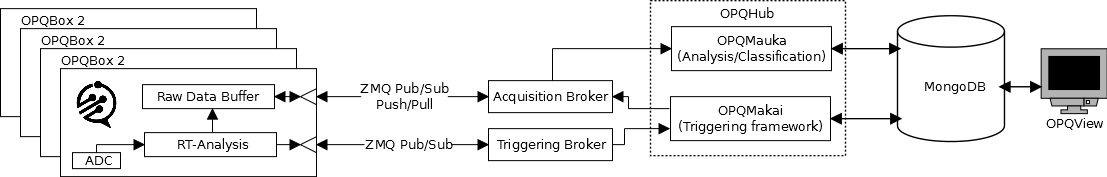
\includegraphics[width=0.9\textwidth]{img/system-diagram.png}
  \end{center}
  \caption{Block diagram of the OPQ Power Quality monitoring system.}
  \label{fig:opq:1}
\end{figure}

Open Power Quality (OPQ) power quality monitoring network utilizes residential power quality meters, called OPQ Boxes, in order to detect anomalies in the electricity distribution across the Oahu power grid.
In addition to OPQ Boxes, the OPQ project utilizes cloud-based aggregation services for power quality event detection, classification and display.
The block diagram of the OPQ network is shown in Figure~\ref{fig:opq:1} .

The major components of OPQ are:
\begin {itemize}
	\item OPQ Box: an in-house designed, open source power quality meter that conforms to Napali Framework requirements for the "source".
	\item Makai: data aggregation and event detection service that conforms to the Napali Framework requirements for the "sink"
	\item Mauka: event analysis and classification service.
\end {itemize}

The following sections describe the OPQ network components, services and protocols.

\section{OPQ Box}\label{sec:opq-box}

OPQ Box is an in-house designed power quality meter which focuses on providing the means for cheap, extensible and accurate residential power quality measurements.
The block diagram of the current revision of OPQ Box, OPQ Box2 is shown in the Figure~\ref{fig:opq:1:1}.
A complete device in an acrylic enclosure is shown in Figure~\ref{fig:opq:1:2}.

\begin{figure}[h]
	\centering
	\begin{subfigure}{.5\textwidth}
	  \centering
	  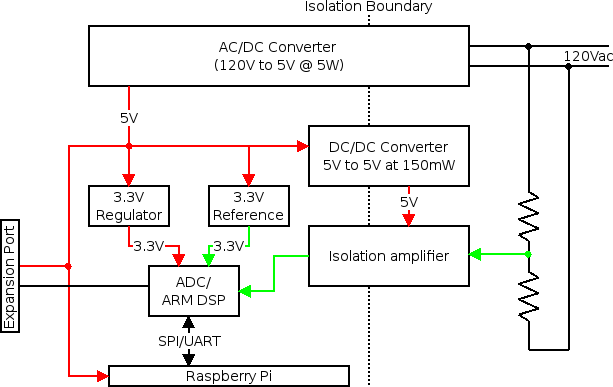
\includegraphics[width=0.9\linewidth]{img/opqbox_diagram.png}
	  \caption{OPQ Box2 Block Diagram.
	  The power path is in red, signal path is in green and the digital IO is in black.}
	  \label{fig:opq:1:1}
	\end{subfigure}%
	\begin{subfigure}{.5\textwidth}
	  \centering
	  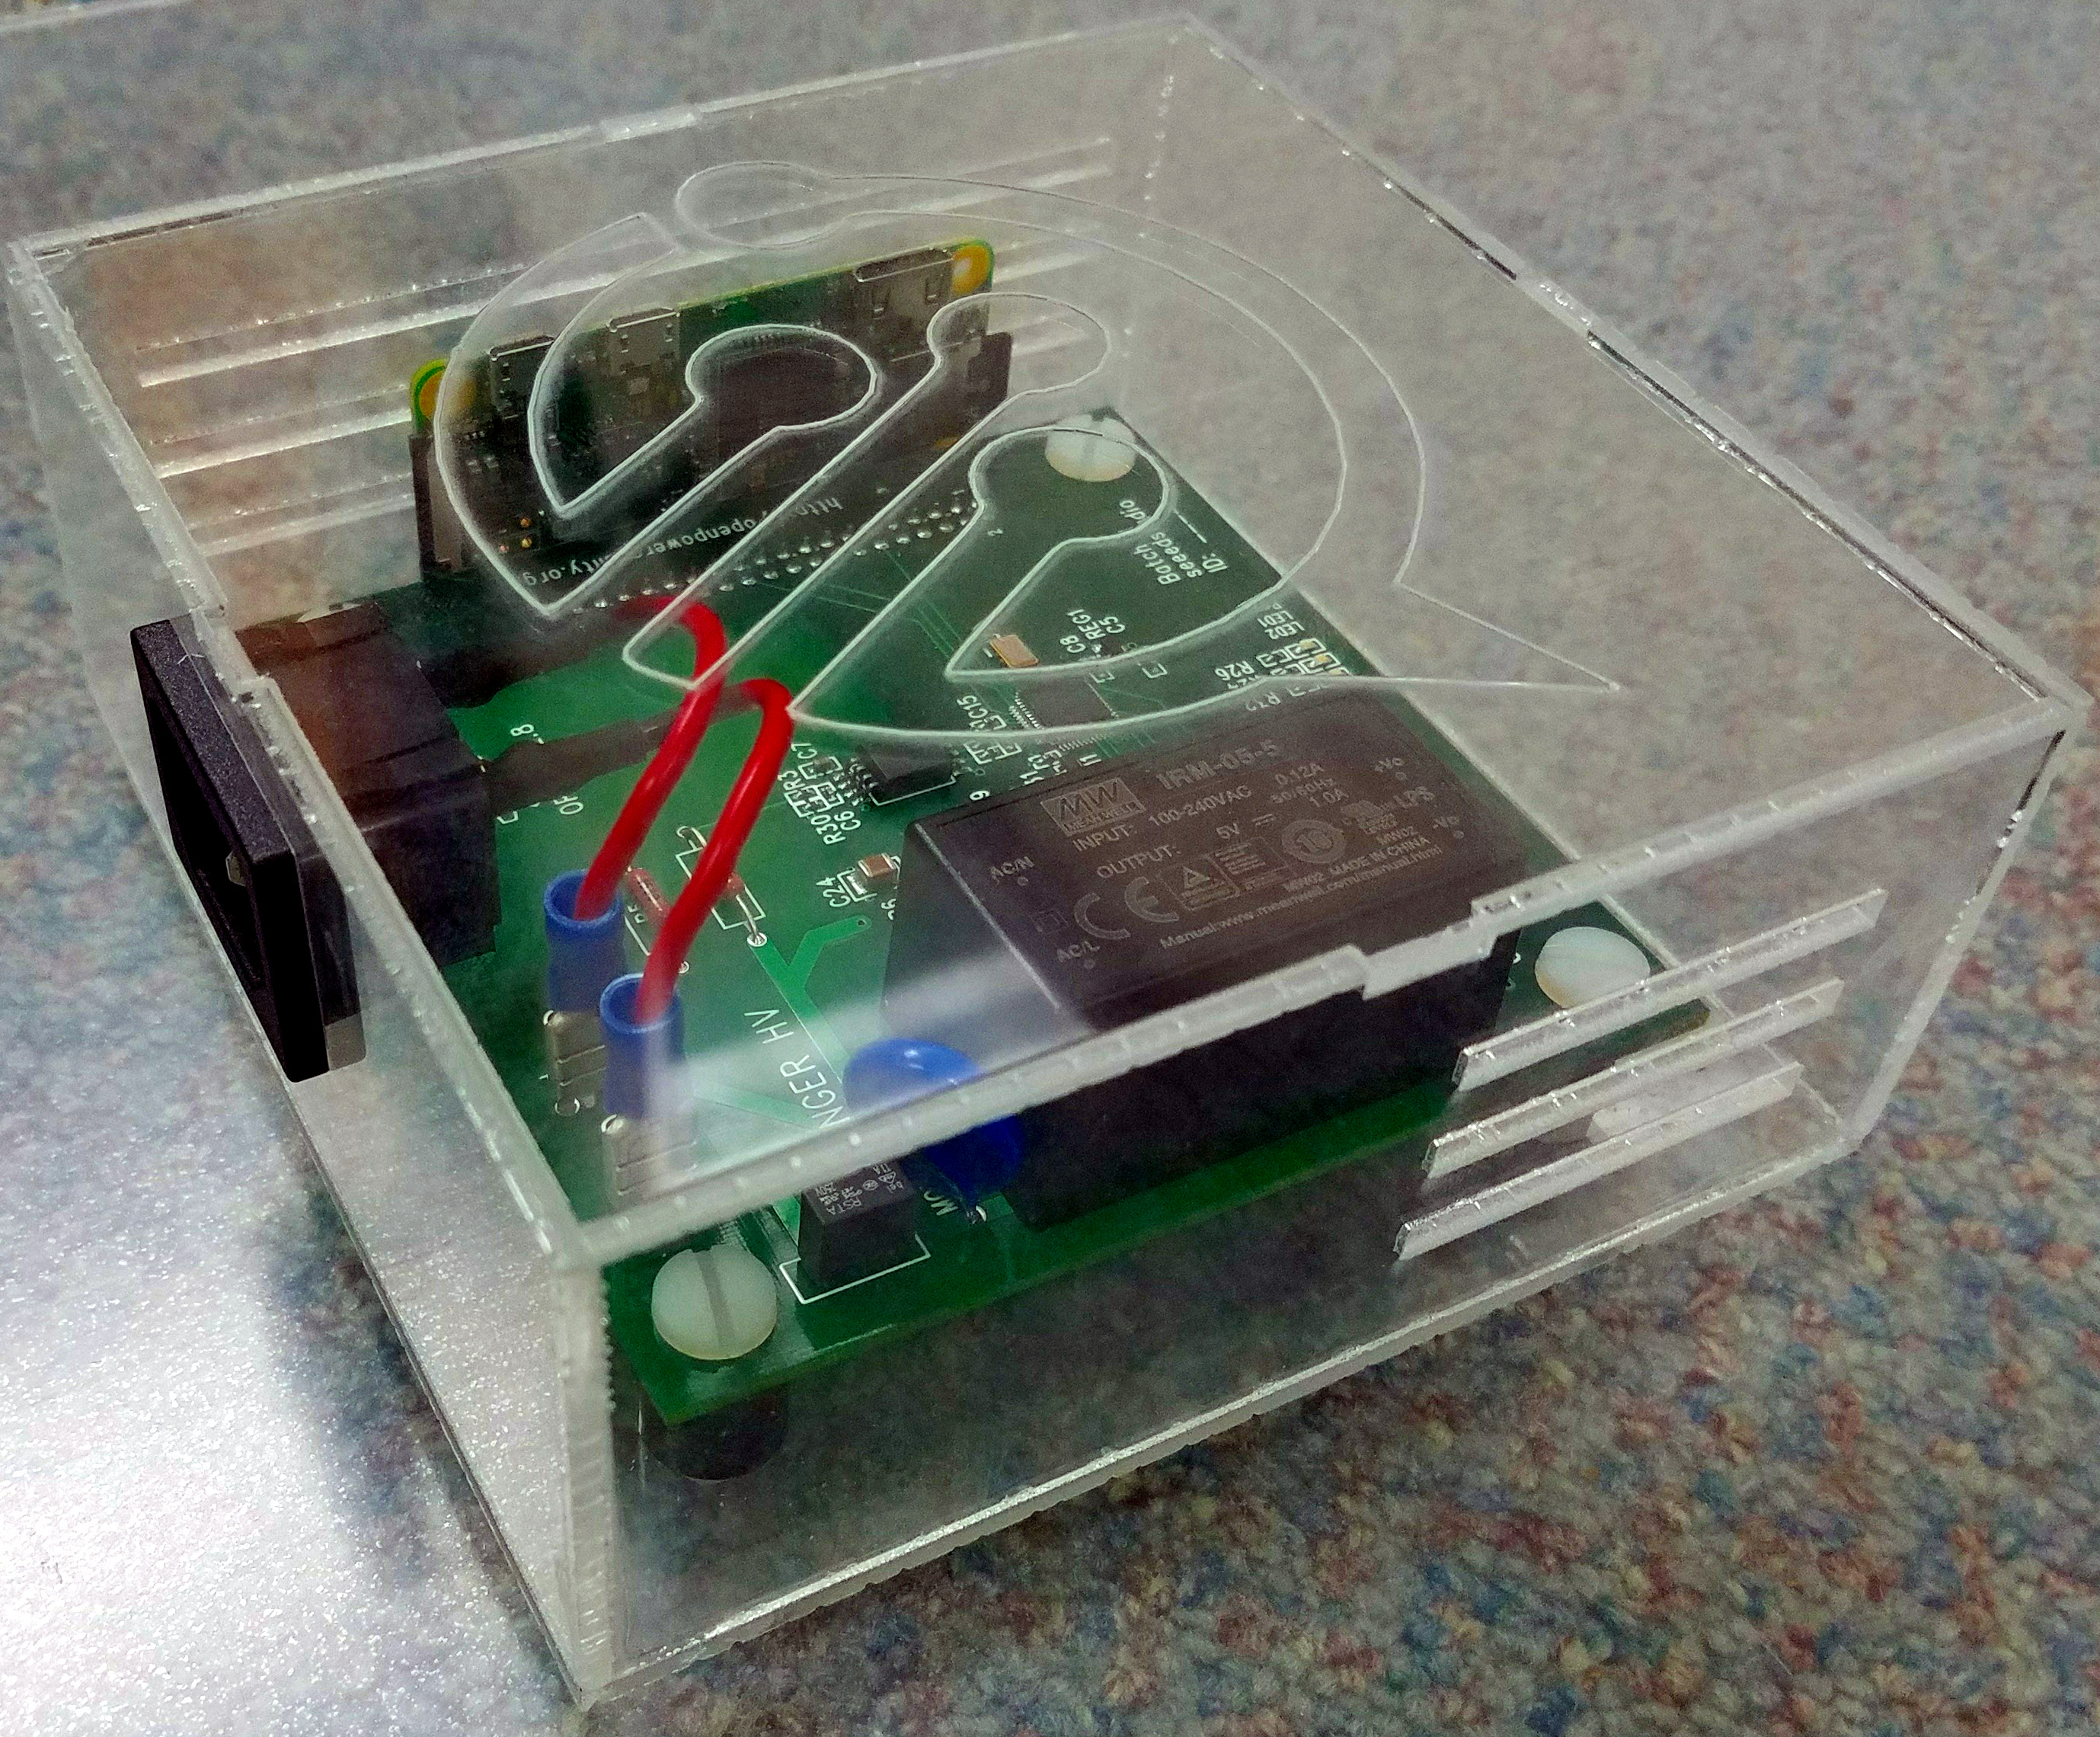
\includegraphics[width=0.7\linewidth]{img/opqbox_photo.jpg}
	  \caption{OPQ Box2 in an acrylic enclosure.}
	  \label{fig:opq:1:2}
	\end{subfigure}
	\caption{(a) OPQ Box2 block diagram and (b) production OPQ box ready for deployment}
	\label{fig:opq:2}
\end{figure}

\subsection{Hardware}\label{subsec:hardware}

The power system of the OPQ box2 electrically isolates most of the device from the AC mains power.
An isolated AC-DC converter generates $5V_{dc}$ from the mains $120V_{ac}$.
5V is used to power the Raspberry Pi, equipment connected to the expansion port, 3.3V regulators and voltage reference and an isolated DC/DC converter.
3.3V is used to power the isolated end of the isolation amplifier as well as the STM32F3 analog to digital converter/digital signal processor (ADC/DSP).
The hot side of the isolation amplifier is powered from the isolated DC/DC converter.
This allows OPQ box to function with the battery attached to the expansion port, so that it may retain data and continue to operate during a power outage.


The analog signal path of the OPQ Box2 is complicated by the fact that the STM32F3 ADC/DSP is electrically isolated from the mains power.
A previous iteration of the OPQ Box, OPQ Box1, overcame this by employing small circuit board mount isolation transformer.
Unfortunately it was found that the frequency response of these transformers varied wildly between individuals, thus incurring a lengthy calibration process for each device.
Design on the OPQ Box2 solved this issue by using an AMC1100 isolation amplifier as the isolation component.
Internally AMC1100 consists of a single die comprised of a $\Sigma\Delta$ analog to digital and digital to analog converters.
These converters are separated by a silicon glass region on the integrated circuit which acts as a coupling capacitor.
Since the signal passes the isolation boundary as a $\Sigma\Delta$ encoded digital signal, it incurs no distortion and no additional calibration is required.
In order to match the dynamic range of the AMC1100 the $120V_{ac}$ is passed through the resistor divider to attenuate it to $120mV_{ac}$.
The input and output of the isolation amplifier is filtered with a passive first order anti-aliasing filter.
Isolated signal is then digitized via a 16bit ADC of the STM32F3 DSP at $12 KSps$, which gives 200 data samples per grid cycle.
Internally digitization process runs asynchronously with the respect to the the DSP CPU, in order to minimize timing jitter.
It was verified that the sampling jitter of the ADC is less then 1us, however due to limited precision of equipment an exact figure was not established.
Data stream in its digital form is transfered to the Raspberry Pi single board computer (SBC) for analysis.

\begin{figure}[h]
  \begin{center}
  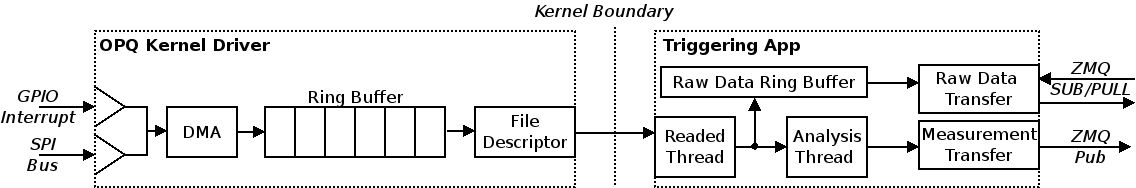
\includegraphics[width=0.9\textwidth]{img/opqbox_software.png}
  \end{center}
  \caption{Block diagram of the OPQ Box 2 software stack.}
  \label{fig:opq:3}
\end{figure}

Raspberry Pi SBC is responsible for signal analysis and anomaly detection.
The Raspberry Pi model used in OPQ Box is the Pi Zero W equipped with 256MB of main memory and a single core 1GHz ARM11 CPU. Furthermore, Pi Zero W is equipped with an on-board 802.11n WIFI transceiver, which removes the need for an external WIFI dongle used in previous OPQ Box devices.
\subsection{Software}\label{subsec:software}
The software stack of the Raspberry Pi aims to deliver a full featured power quality analysis framework despite its rather limited hardware capabilities.
A block diagram of the software stack is shown in Figure~\ref{fig:opq:3}.
Digital data is transferred from the DSP to the Raspberry Pi via Serial Peripheral Interface, with the Pi acting as the master and the DSP as a slave device.
A hardware interrupt line is used to inform Pi software that the DSP is ready for the data transfer.
During the initial design of the OPQ box 2 software, SPI data transfer was attempted in userland.
However due to the lack of support for DMA in the SPI kernel-to-userland bridge, a large portion of the CPU time was spent facilitating data transfer, resulting in degraded analysis performance as well as missed data samples.
Current revision of the OPQ Box 2 software stack utilizes a kernel driver for management of SPI bus.
Internally OPQ driver maintains a ring buffer of 16 windows each 200 data samples in size.
Upon the receiving the interrupt for the DSP, the CPU sets up the DMA transfer and the DMA engine transfers a 200 sample window into the kernel memory without CPU interaction.
This scheme requires the CPU to only service 60 interrupts a second, with each interrupt requiring on the order of 100 instructions, yielding the CPU utilization of less then $1\%$ in normal operation.
Userland applications communicate with the kernel driver using a file descriptor, where every $write$ system call yields 200 samples of raw waveform.
Thus the smallest window that a userland application may process is a single AC cycle of the grid mains.

Userland component of the OPQ Box 2 software is a multi-threaded extensible analysis framework called Triggering.
The reader thread is responsible for transferring and accumulating data from the kernel driver.
The smallest data buffer that the Triggering application processes at any given time is 10 grid cycles or 2k samples.
Once the cycles are transfered to the userland and timestamped, they are passed to the analysis thread for feature extraction, as well as to the Raw Data Ring Buffer (RDRB).
Since internally all data is addressed using shared pointers, during data duplication no copying is required.
RDRS is capable of buffering up to an hour of historic data before it's overwritten resulting in the RDBS maximum size of 100MB.

Analysis thread of the Triggering application performs feature extraction of the raw data windows of 2000 samples.
Four metrics are extracted from the data stream:
\begin{itemize}
	\item Fundamental frequency.
	\item RMS Voltage.
	\item Total Harmonic Distortion.
	\item Transient.
\end{itemize}

\subsection{Fundamental Frequency}\label{subsec:fundamental-frequency}

Fundamental frequency is calculated by computing the zero crossings of the AC waveform.
Since a sinusoid has two zero crossings for a full cycle the frequency can be calculated as:
\begin{equation} \label{eq:1}
 f = \frac{1}{\frac{2}{n}\sum\limits_{k=0}^{k=n}{\Delta t_{k}}}  
\end{equation}

\begin{figure}[h]
	\centering
	\begin{subfigure}{.5\textwidth}
	  \centering
	  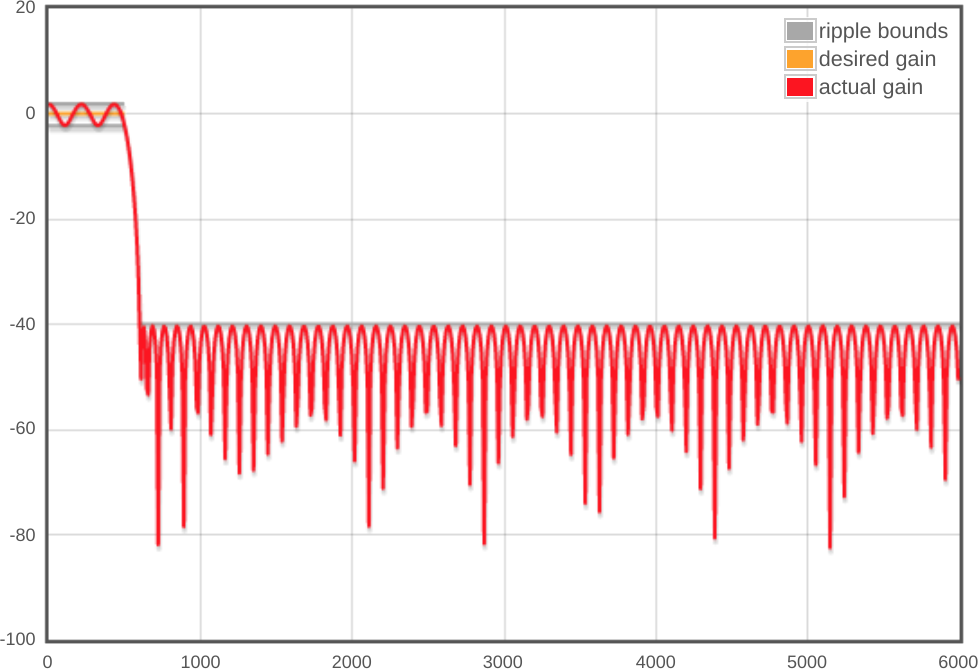
\includegraphics[width=0.9\linewidth]{img/filter1_gain.png}
	  \caption{}
	  \label{fig:opq:4:1}
	\end{subfigure}%
	\begin{subfigure}{.5\textwidth}
	  \centering
	  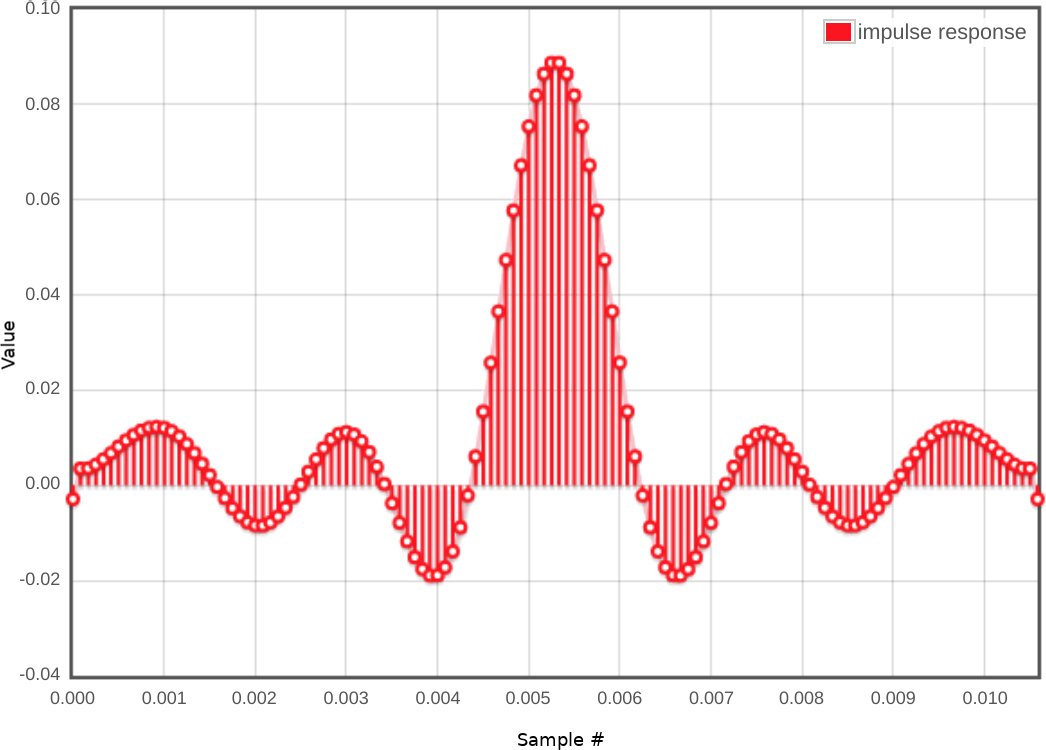
\includegraphics[width=0.9\linewidth]{img/filter1_response.png}
	  \caption{}
	  \label{fig:opq:4:2}
	\end{subfigure}

	\begin{subfigure}{.5\textwidth}
	  \centering
	  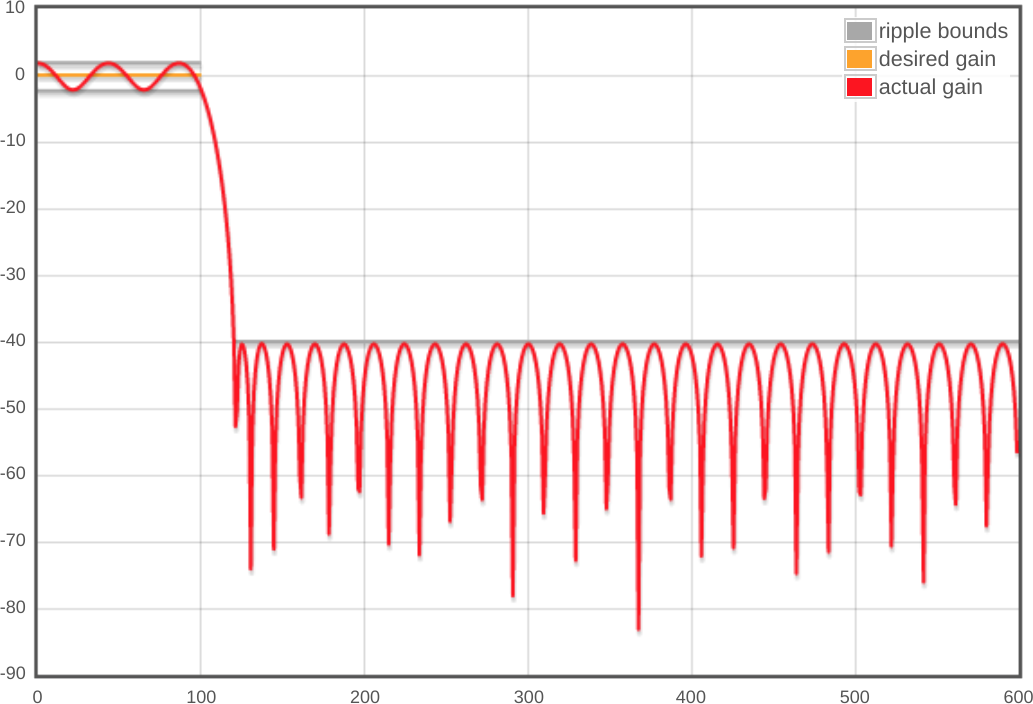
\includegraphics[width=0.9\linewidth]{img/filter2_gain.png}
	  \caption{}
	  \label{fig:opq:4:3}
	\end{subfigure}%
	\begin{subfigure}{.5\textwidth}
	  \centering
	  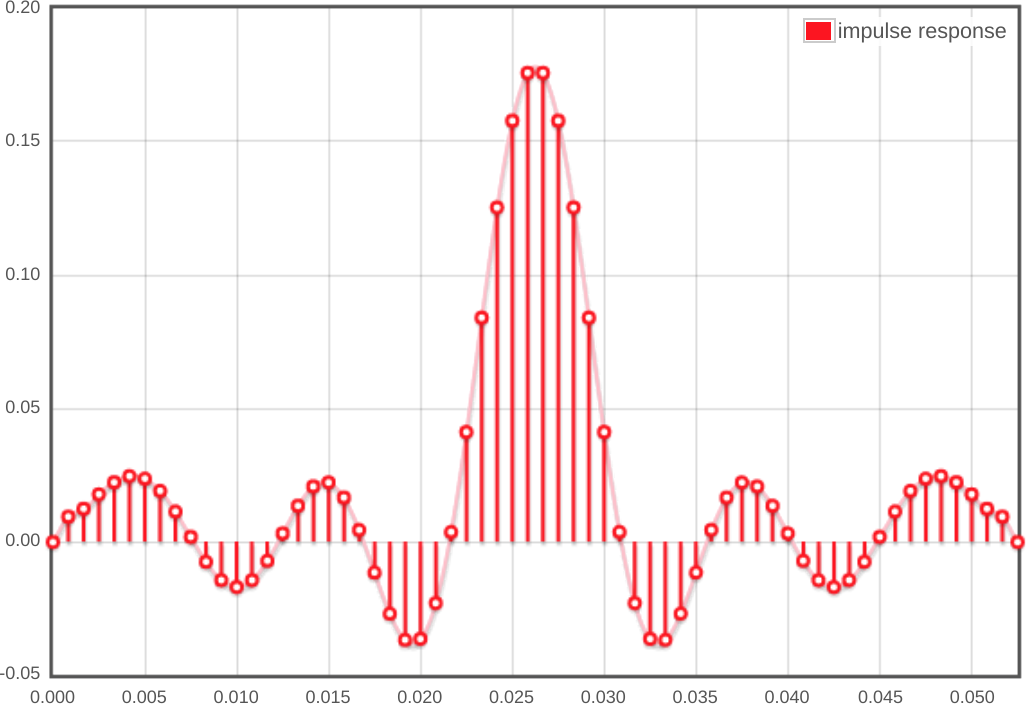
\includegraphics[width=0.9\linewidth]{img/filter2_response.png}
	  \caption{}
	  \label{fig:opq:4:4}
	\end{subfigure}
	\caption{Filters used for mains frequency calculation. (a) Downsampling filter gain. (b) Downsampling filter impulse response. (c) Lowpass filter gain. (d) Lowpass filter impulse response.}
	\label{fig:opq:4}
\end{figure}

Where the $\Delta t_{k}$ is the k'th time between two adjacent zero crossings.
In order to improve the accuracy of the frequency calculation one must first filter out as much of out of band noise as possible.
Since our sampling rate is quite high (12kSps) and the fundamental frequency is quite low (60Hz) it is very computationally expensive to perform this filtering in a single step.
Instead filtering is accomplished via a set of two finite impulse response (FIR) filters shown in Figure~\ref{fig:opq:4:2} and~\ref{fig:opq:4:4}.
First the Down sampling filter is applied to the raw waveform, which results in the frequency response shown in Figure~\ref{fig:opq:4:1}.
As is evident by the plot the frequency content of the result is 0-600Hz, Thus it can be downsampled to the $\frac{N}{10}$, or 200 samples without aliasing.
Next the low pass filter is applied to the downsampled waveform with the frequency response shown in Figure~\ref{fig:opq:4:3}.This resulting frequency content is 0-100Hz, thus all of the higher frequency harmonics and noise are removed.
Finally the twice filtered downsampled waveform is used to estimate the fundamental frequency according to the Equation~\ref{eq:1}.
The zero crossings themselves were calculated by using linear interpolation between two points which bracket the time axis.

All electrical generation systems connected to the grid run synchronously with each other, meaning that while small variations in voltage are common across locations, the fundamental frequency and phase must remain strictly in sync.
This effect is demonstrated in Figure~\ref{fig:opq:5}, which is a frequency fluctuation event recorded on November 8 2017.
While the two devices were separated by ten miles, their frequency measurements track closely together.

\begin{figure}[h]
	\centering
	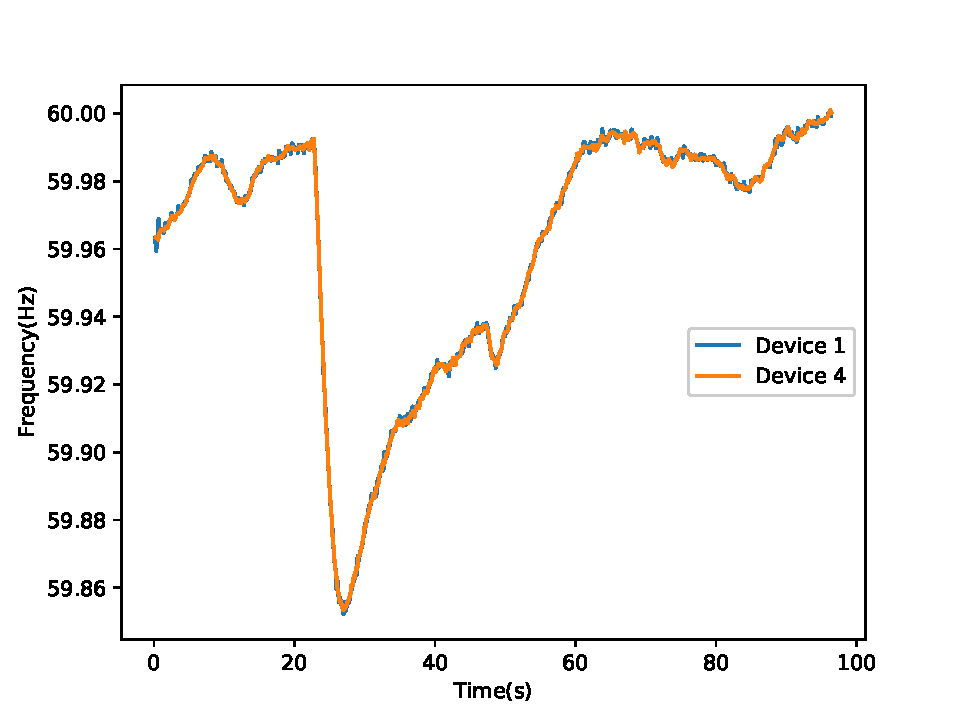
\includegraphics[width=0.6\linewidth]{img/frequency_two_devices.pdf}
	\caption{Frequency measurement across two devices recorded during a lighting strike.}
	\label{fig:opq:5}
\end{figure}

\subsection{Root Mean Square Voltage}\label{subsec:root-mean-square-voltage}

Root mean square voltage ($V_{rms}$) in electrical power is the equivalent value of DC voltage which would dissipate the same power in the resistive load. $V_{rms}$ is a convenient measure for detecting voltage sags and swells, since they result in nominally higher and lower computed value.
For the sinusoidal signal $V_{rms}$ can be calculated from the peak to peak value ($V_{pp}$) as:
\begin{equation} \label{eq:2}
	V_{rms} = \frac{V_{pp}}{2\sqrt{2}}
\end{equation}
It is common for multimeter to employ the equation above for computing $V_{rms}$.
However this equation is only valid for a perfect sinusoid, and thus does not result in a suitable metric for identifying power quality disturbances.
Instead OPQ Box 2 computes $V_{rms}$ as follows:
\begin{equation} \label{eq:3}
	V_{rms} = \sqrt{\frac{1}{n}\sum\limits_{k=0}^{k=n}V_{k}^{2}}
\end{equation}
Similarly to the frequency calculation OPQ Box 2 usees a 10 cycle window for a single $V_{rms}$ calculation, however unlike the frequency calculation the input is not filtered a priori.
An example of a power quality disturbance which exhibits low $V_{rms}$ is shown in Figure~\ref{fig:opq:6:1} and~\ref{figopq:6:2}.
These disturbances are the result of a lighting strike recorded by two OPQ Box 2 devices on Nov 1, 2017.

\begin{figure}[h]
		\centering
	\begin{subfigure}{.5\textwidth}
	  \centering
	  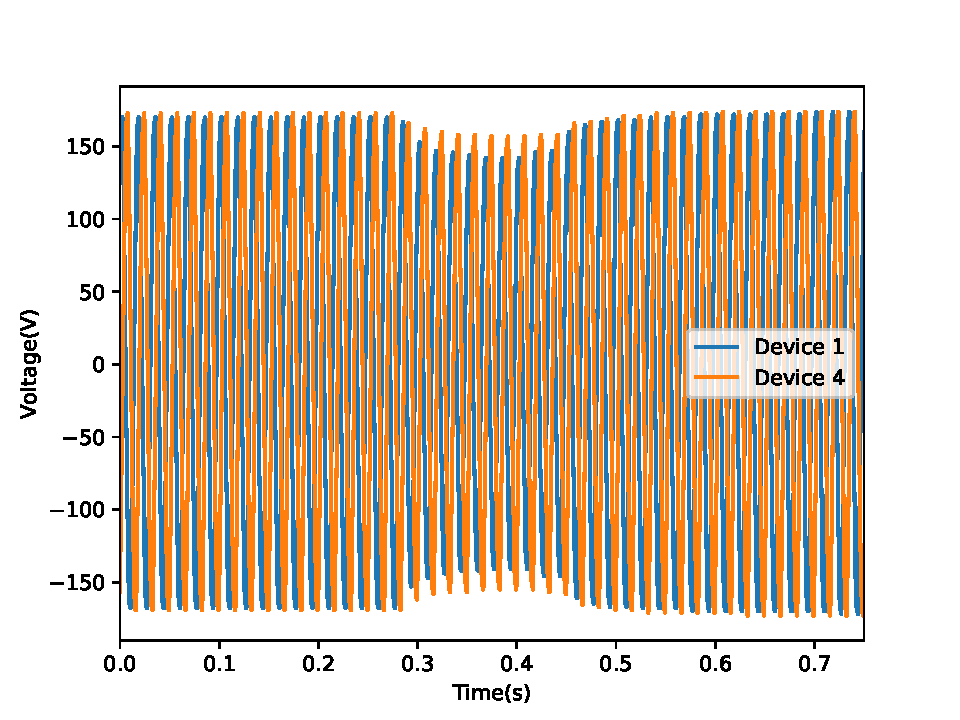
\includegraphics[width=0.9\linewidth]{img/voltage_sag.pdf}
	  \caption{}
	  \label{fig:opq:6:1}
	\end{subfigure}%
	\begin{subfigure}{.5\textwidth}
	  \centering
	  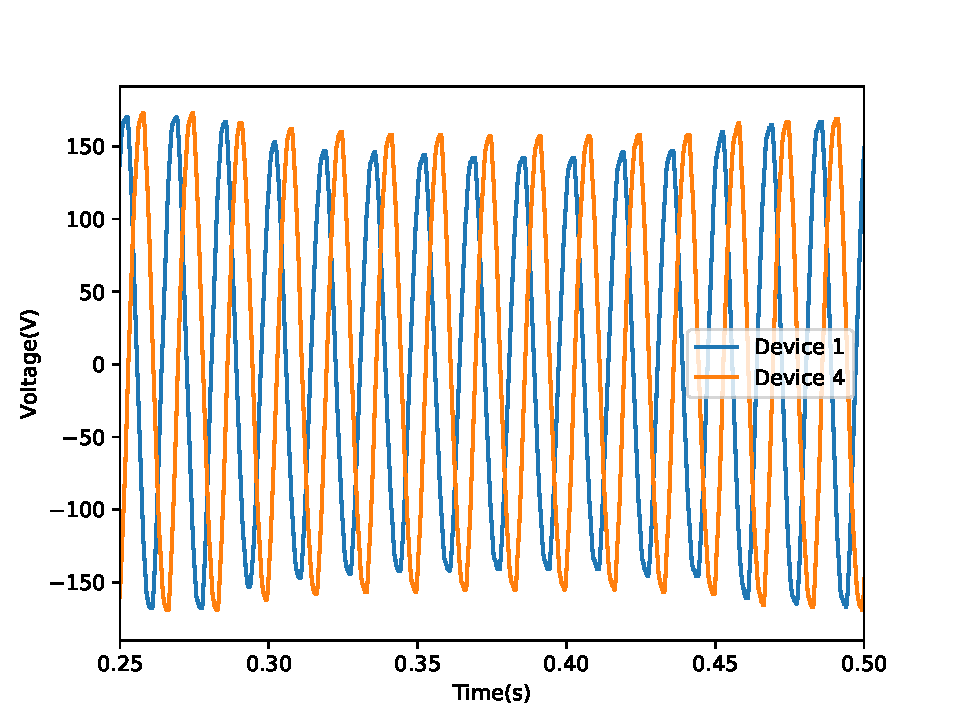
\includegraphics[width=0.9\linewidth]{img/voltage_sag_zoomed_in.pdf}
	  \caption{}
	  \label{fig:opq:6:2}
	\end{subfigure}
	\caption{A lightning strike recorded by two OPQ Box 2 devices separated by 10 miles. (a) A lightning strike manifested as $V_{rms}$ dip which lasted 11 cycles. (b) As a consequence of using NTP these devices have $\frac{1}{2}$ cycle mismatch in reported timestamps.}
	\label{fig:opq:6}
\end{figure}


\subsection{Total Harmonic Distortion}\label{subsec:thd}
OPQBox calculates THD using industry standard methodology.
In the power delivery industry THD is defined as:
\begin{equation} \label{eq:4}
THD = \frac{\sqrt{\sum{V_{n}^2}}}{V_{f}}*100\%
\end{equation}
Where $V_{f}$ is the fundamental 60Hz power and $V_{n}$ is the power at $n^{th}$ harmonic.
It should be noted that in the power quality domain THD is expressed as a percentage as opposed to $\frac{dB}{\sqrt{Hz}}$ as used in other disciplines.
Operationally, OPQBox computes THD for 10 cycles of the fundamental frequency.
First an FFT transforms the real voltage samples into it's frequency components.
Next, the square of the harmonic bins is accumulated and scaled by the magnitude of the fundamental power.

\begin{figure}[h]
	\centering
	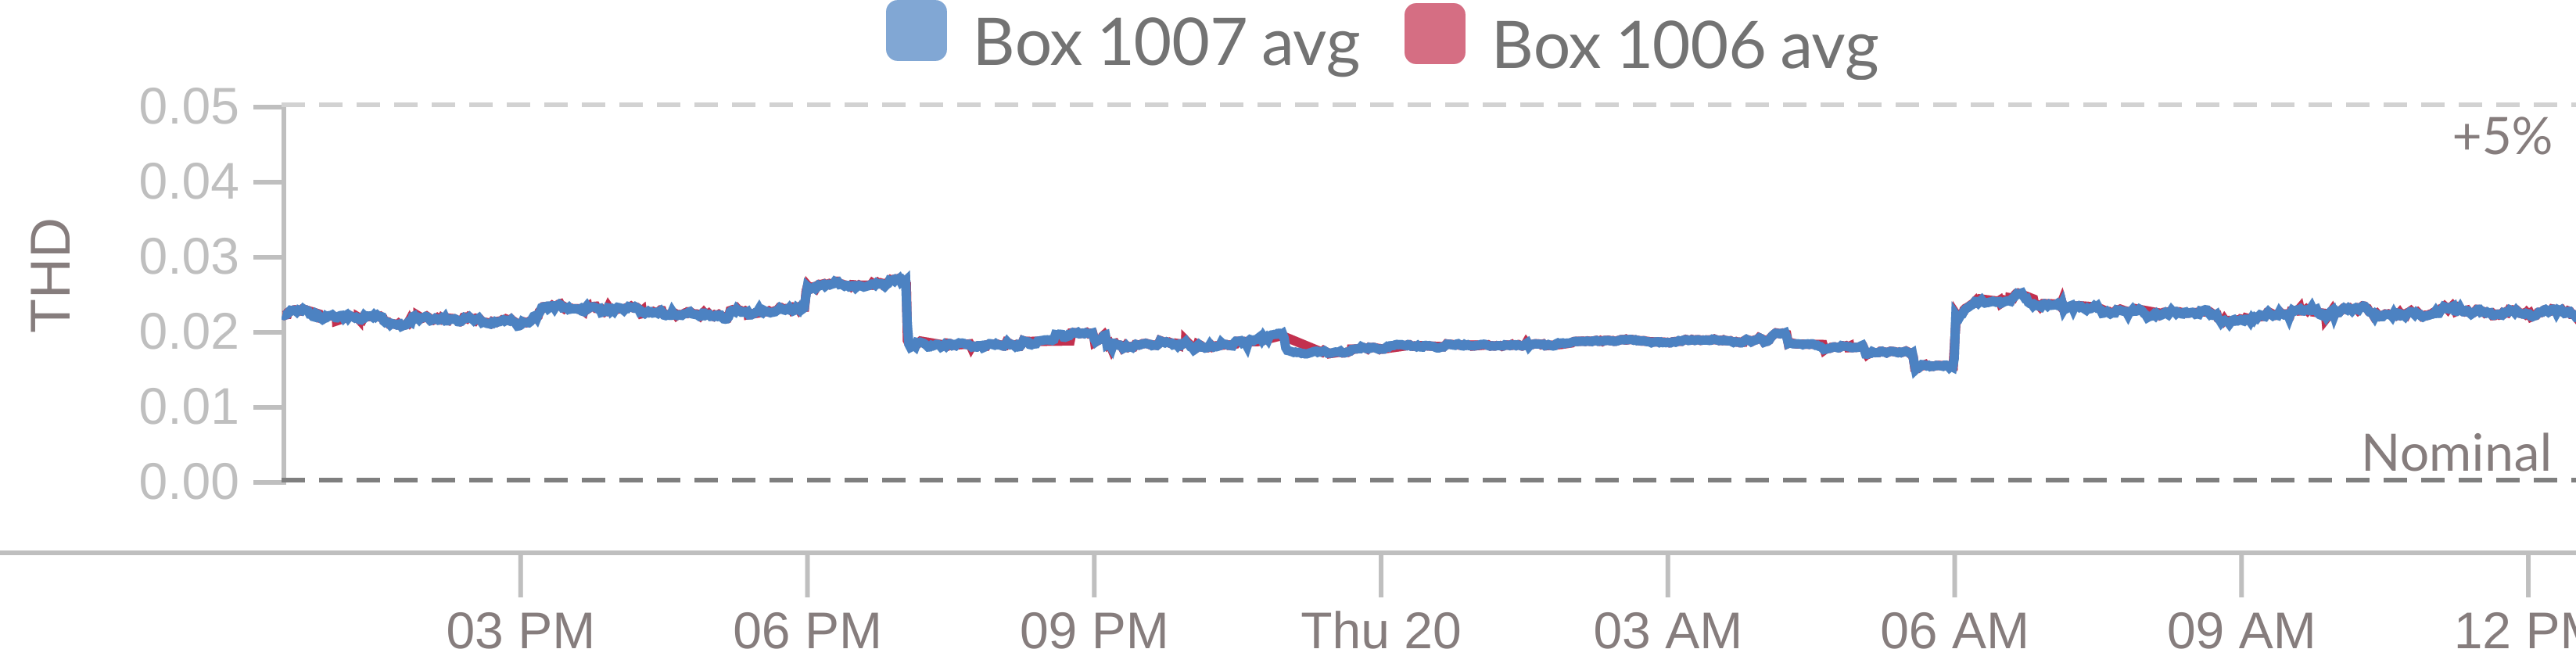
\includegraphics[width=1\linewidth]{img/thd_two_devices_24_hours.png}
	\caption{A common THD trend across two OPQBox devices each deployed in the two Flexible Response to Ongoing Growth buildings on UH campus.}
	\label{fig:opq:7}
\end{figure}

Figure~\ref{fig:opq:7} shows a common trend observed by all OPQBox devices installed on the UH campus.
For clarity only two devices are shown.
It is assumed that the large drop observed daily from approximately 6am to 6pm corresponds to the automatic response of the power delivery system to the reactive power in the grid, by deploying a large capacitor bank to compensate for the current phase lag.

\subsection{Transient Detection}\label{subsec:transient-detection}

OPQBox transient detection is performed via filtering out of the fundamental frequency via an FIR high pass pass filter and searching for a maximum value in the remainder.
The high pass filter has a cutoff of $400Hz$, and the filter coefficients and response are shown in Figure~\ref{fig:opq:8:2} and Figure~\ref{fig:opq:8:1} respectively.
The result of the high pass filter operation is shown in Figure~\ref{fig:opq:8}.
Figure~\ref{fig:opq:8:3} shows a synthetic signal generated via a SDG1025 signal generator and fed into the OPQBox.
This signal contains a $5V_{pp}$ transient injected at 11ms.
Filtered signal is shown in Figure~\ref{fig:opq:8:4}, with the fundamental removed and the transient preserved.
OPQBox scans for the highest sample in the filtered waveform and uses its magnitude as a transient detection metric.


\begin{figure}[h]
	\centering
	\begin{subfigure}{.5\textwidth}
		\centering
		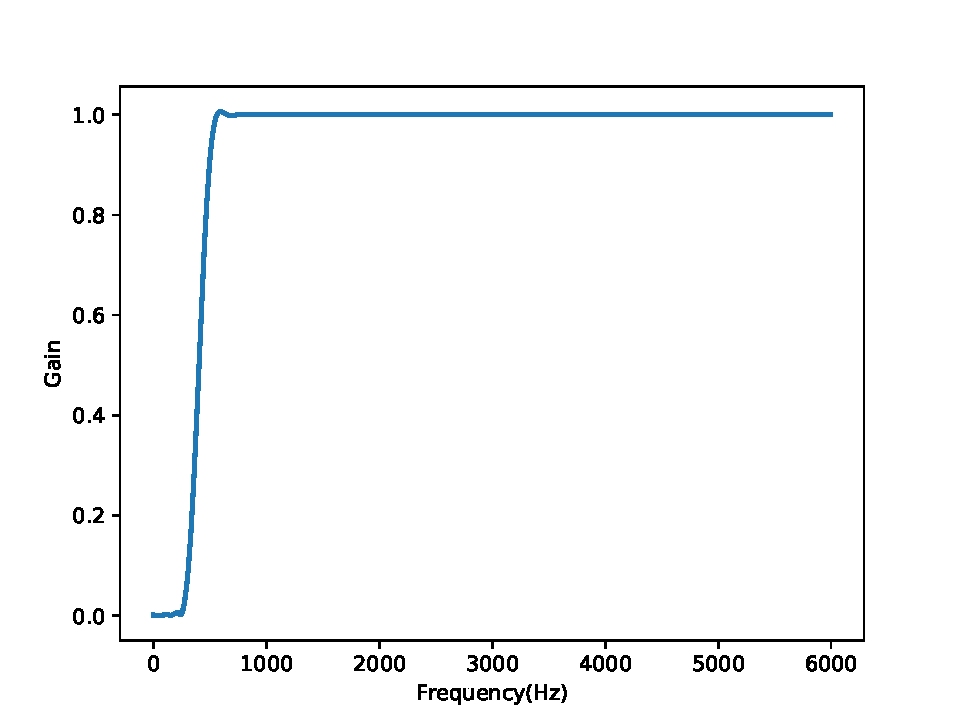
\includegraphics[width=1\linewidth]{img/thd_hpf_resp.pdf}
		\caption{}
		\label{fig:opq:8:1}
	\end{subfigure}%
	\begin{subfigure}{.5\textwidth}
		\centering
		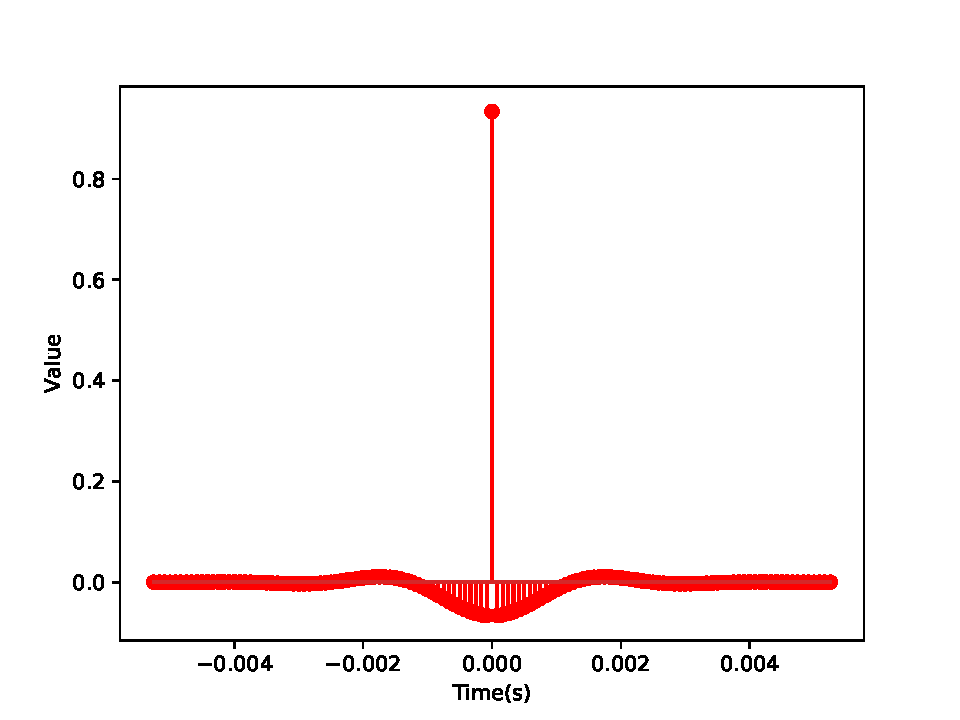
\includegraphics[width=1\linewidth]{img/thd_hpf.pdf}
		\caption{}
		\label{fig:opq:8:2}
	\end{subfigure}

	\begin{subfigure}{.5\textwidth}
		\centering
		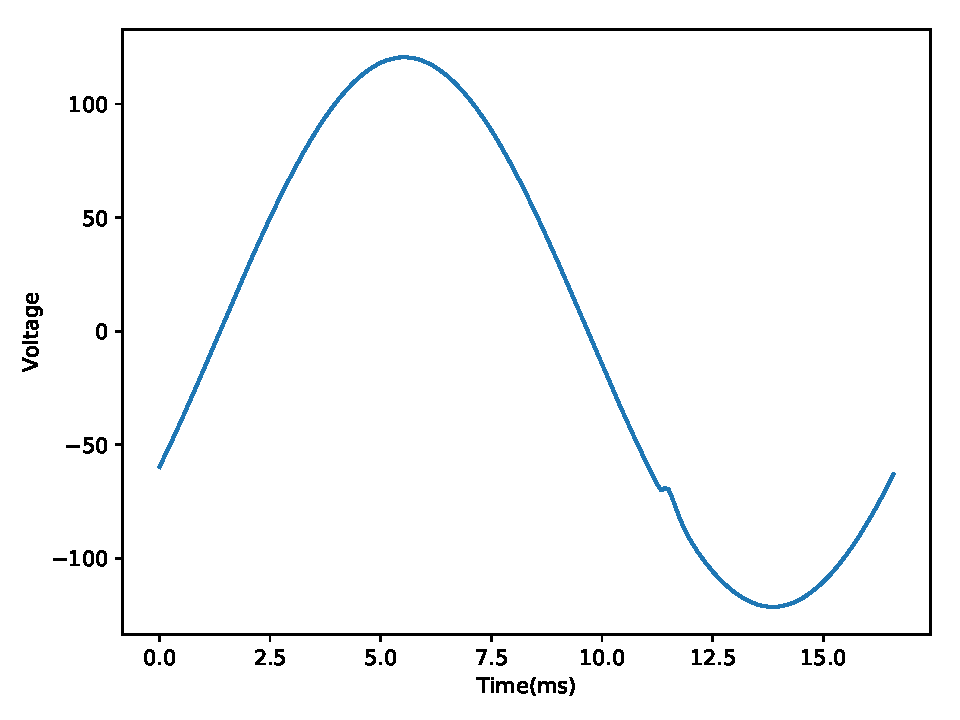
\includegraphics[width=0.86\linewidth]{img/box_eval/5v_transient.pdf}
		\caption{}
		\label{fig:opq:8:3}
	\end{subfigure}%
	\begin{subfigure}{.5\textwidth}
		\centering
		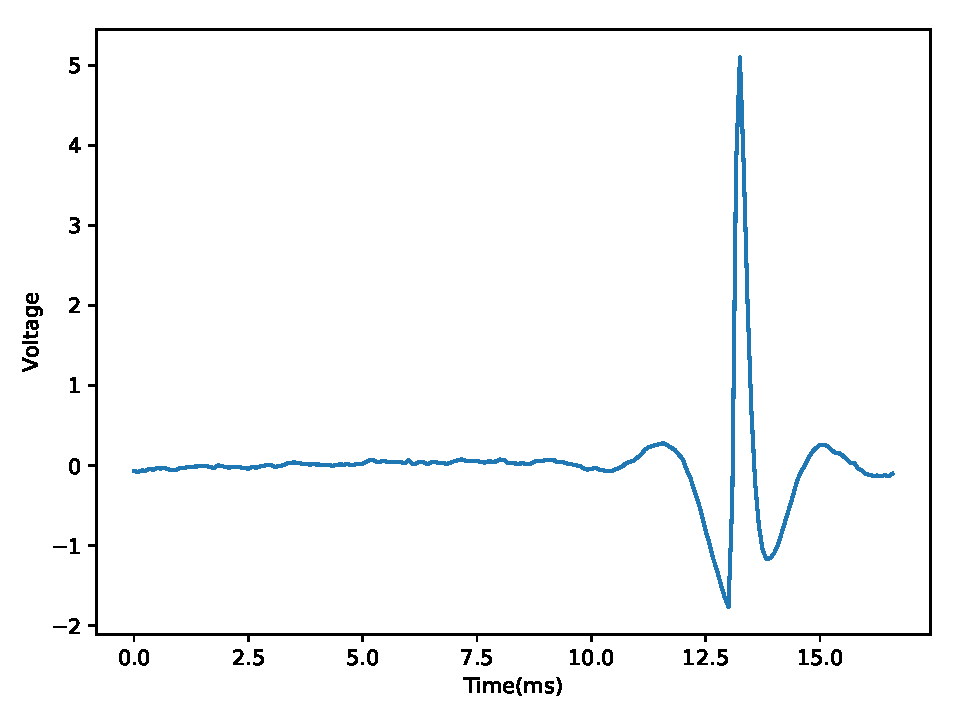
\includegraphics[width=0.86\linewidth]{img/box_eval/5v_transient_filtered.pdf}
		\caption{}
		\label{fig:opq:8:4}
	\end{subfigure}
	\caption{THD detection filtering. (a) Filter gain. (b) Filter response. (c) A 5V transient superimposed onto a fundamental. (d) Filter result from (c).}
	\label{fig:opq:8}
\end{figure}

It should be noted, that this transient detection method is susceptible to THD fluctuations, since any harmonic above $400Hz$ will remain in the filtered waveform.
However, since the THD information is transmitted along with the transient detection metric, they can be correlated in downstream transient detection.
This effect can be seen in Figure~\ref{fig:opq:9}.
This figure shows both the THD and transient detection metric during a transient event.
A small transient of approximately 1.6V was observed occurring at 2600s, while the sensitivity of the transient metric is clearly visible, particularly between 3000s and 4500s.

\begin{figure}[h]
	\begin{center}
		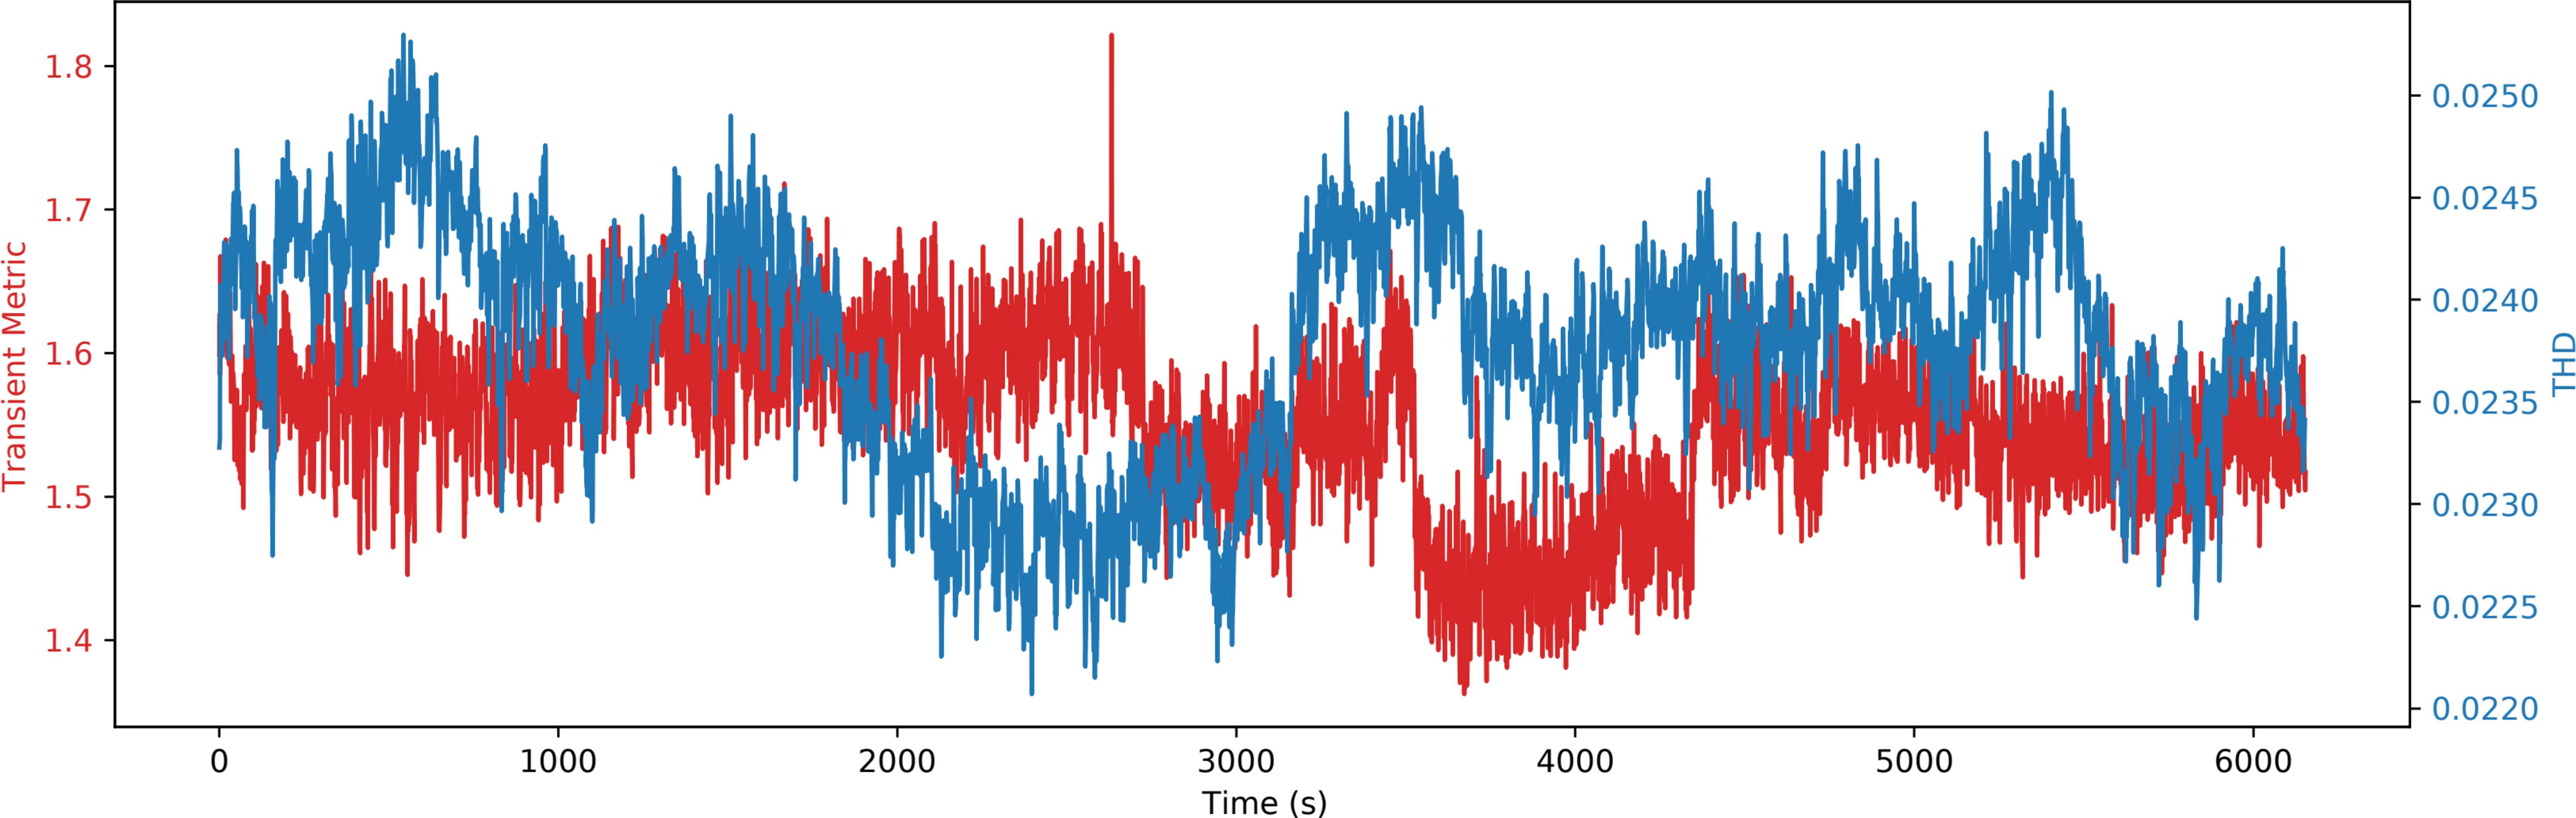
\includegraphics[width=1\textwidth]{img/trans_thd_det.pdf}
	\end{center}
	\caption{THD and Transient detection metric.}
	\label{fig:opq:9}
\end{figure}

\subsection{Network Communication}\label{subsec:network-communication}

Computed fundamental frequency and $V_{rms}$ are transmitted to the Makai service for aggregation.
Data transmission is handled using 0MQ software stack with Curve25519 elliptic curve encryption.
Each device holds a unique of private and public keys, as well as the servers public key, allowing both the Makai service and the OPQ Box 2 to verify it's peer.
Internally metrics transmission uses 0MQ's PUB/SUB protocol.
This protocol is a publish subscribe one to many topology, with each message containing the topic, and a payload.
Additionally 0MQ pub-sub topology allows for multiple sub peers with subscriptions forwarder to the publisher automatically via a side channel.
This allows for the aggregation service to be spread across multiple nodes, with minimal network overhead.

If the aggregation service determines that an anomaly has occurred, it is able to request raw waveform from the OPQ Box 2 RDRB via a separate 0MQ pub sub channel.
If the RDRB buffer contains data for the requested temporal range, OPQ Box 2 transmits the available data to the aggregation service via a push pull 0MQ channel.
Protobuf message serialization is used to encode messages across the OPQ ecosystem.


In order to make a distributed measurement, all of the OPQ Boxes on the OPQ network need to maintain an accurate time reference.
Time synchronization across multiple OPQ Boxes is accomplished using the Network Time Protocol.
The expansion port of the OPQ Box 2 supports a GPS receiver, however using it is detrimental to the OPQ Box 2 utility.
GPS receivers require line of sight to the sky, and since the with out on-board real-time clock, every power interruption requires a GPS cold start.
NTP performance has been verified against GPS resulting in time error of $8ms\pm 5ms$ which is typical for NTP running over the Internet with a close by NTP server.
This error is visualized in a Figure~\ref{fig:opq:6:2}.
With a large coincidental $V_{pp}$ drop across two devices, a 7ms phase error is clearly visible.


\section{OPQ Makai}\label{sec:opq-makai}

OPQ Makai implements the Napali Framework requirements for a ``sink''.
 It is a distributed extensible microservice framework responsible for receiving the triggering stream from the OPQ Boxes, locating anomalous temporal regions and requesting raw waveform for the anomalous time ranges.
 As evident from the block diagram shown in Figure~\ref{fig:opq:10}, Makai consists of three major components: Acquisition Broker, Triggering Broker, and the Acquisition Service.
\begin{figure}[h]
  \begin{center}
  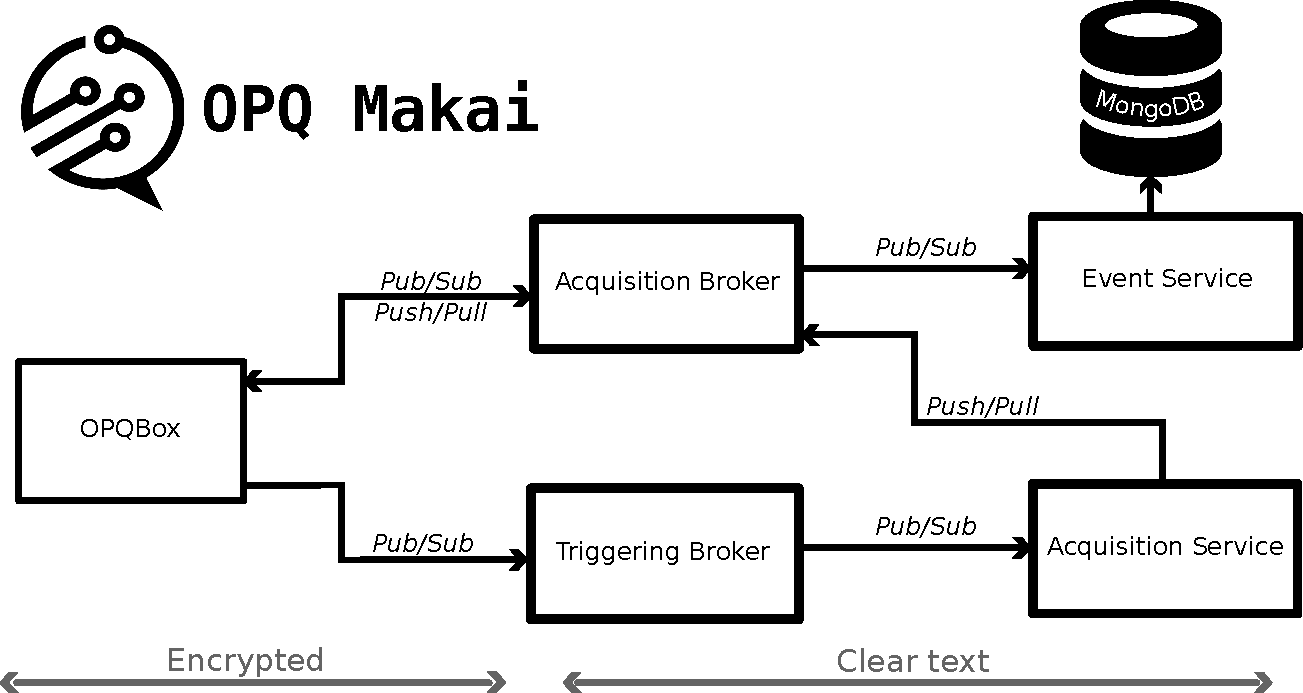
\includegraphics[width=0.6\textwidth]{img/makai_main.pdf}
  \end{center}
  \caption{Block diagram of the OPQ Makai.}
  \label{fig:opq:10}
\end{figure}

\subsection{Triggering Broker}\label{subsec:triggering-broker}

The triggering Broker is perhaps the simplest component of the OPQ Makai system.
The triggering stream generated by the OPQ Boxes is encrypted to preserve users privacy.
In order to minimize the CPU time spent decrypting the data across multiple OPQ services, the Triggering Broker is used to decrypt the data and send clear text measurements across the rest of the OPQ ecosystem.
Triggering Broker uses the 0mq sub socket to receive data form OPQ Boxes, and send, it via a pup socket to any connected client.
Another potential role of the Triggering Broker is load balancing.
Since the 0MQ pub/sub sockets are subscription based, services connecting to the triggering broker can selectively receive measurements only from OPQ Boxes they are interested in.

\subsection{Acquisition Broker}\label{subsec:acquisition-broker}

The Acquisiton Broker manages the two way communication between the OPQ Boxes and the rest of the cloud infrastructure.
Unlike the triggering stream which originates from the OPQ Box, two way communication is always initiated by the cloud services.
Two way communication is realized via a command response interface, where the OPQ service initiates the communication by sending in clear text command to the Acquisition Broker, which then forwards it in the encrypted form to the appropriate OPQ Boxes.
There are three command types which can be handled by the Acquisition Broker:
\begin{itemize}
\item{\textbf{(PING) Ping:}} The ping command is broadcast periodically across all of the OPQ Boxes, in order to monitor the health of the OPQ network.
The OPQ Box response to this command contains diagnostic information, such as the timestamp of the last event requested, ip address and the name and strength of the WIFI network the OPQ Box is connected to.
\item{\textbf{(CMW) Change measurement window:}} This command allows to vary how often a triggering stream message is generated and delivered to the triggering broker.
This is accomplished by varying the length of the temporal window used to derive the triggering metrics.
This allows the OPQ system to analyze a finer grained measurements if a potential anomaly is taking place.

\item{\textbf{(RD) Send raw data:}} This command instructs the OPQ Box to send data from the its raw data buffer to the cloud. 
\end{itemize}

The last command in particular is unique, because its response is trapped by the Acquisition Broker, as opposed to being passed to the agent which initiated communication.
In this case the raw data is serialized and stored in the Mongo database.
Furthermore, the Acquisition Broker notifies all connected agents that a new anomaly has been recorded via a 0mq pub message.

\subsection{Acquisition Service}\label{subsec:acquisition-service}

The Acquisition Service middleware resides in between the Triggering and Acquisition Brokers.
It processes the triggering stream and manipulates it using the \textbf{CMW} command and if an anomaly is suspected requests raw data from boxes via the \textbf{RD} command.
The Acquisition Service app itself does not perform any analysis of the triggering stream.
Instead it provides a loadable plugin interface which allows for a runtime hotplugable analysis.
Since the OPQ Makai core is written in the Rust programing language, the loadable object interface supports supports any programing language with LLVM bindings.
As such OPQ Makai plugins can be developed in C/C++, Rust, or even Lisp.
Currently three plugins are implemented:

\begin{itemize}
\item{\textbf{Print Plugin:}} Prints the triggering stream to the stdout for debugging purposes. 
\item{\textbf{Ketos:}} A Lisp interpreter built on top of the LLVM for manipulating/debugging the triggering stream.
\item{\textbf{Threshold:}} This plugin monitors the triggering stream, while looking for metrics which exceed the user defined thresholds.
If the threshold is crossed, data from all of the OPQ Boxes is requested for the offending time interval via the RD command.
\end{itemize}

\section{OPQ Mauka}\label{sec:opq-mauka}
OPQ Mauka service is responsible for higher level classification and filtering of the anomalies generated by the OPQ Makai.
Since anomalies generation only
relies on the triggering stream features and not raw data, OPQ Makai is not able to ascertain if the anomaly is an actual power quality event, event type, or its severity.
OPQ Mauka on the other hand operates on the raw data, thus it is able to perform high level analysis to meet industry standards for vent classification.
The block diagram of the OPQ Mauka is shown in~\ref{fig:opq:11}.
\begin{figure}[h]
  \begin{center}
  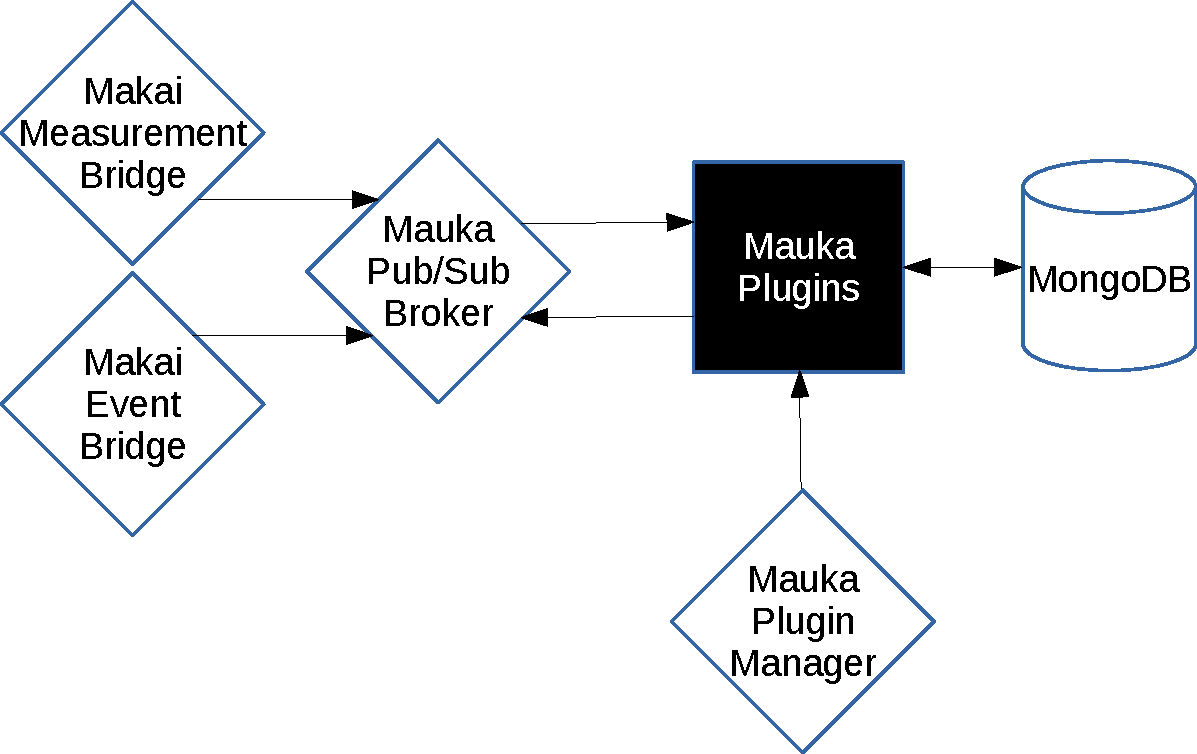
\includegraphics[width=0.6\textwidth]{img/mauka.pdf}
  \end{center}
  \caption{Block diagram of the OPQ Mauka.}
  \label{fig:opq:11}
\end{figure}

Currently OPQ Mauka supports the following classification strategies: 
\begin{itemize}
	\item{\textbf{ITIC}} Power acceptability curve used to classify short term voltage sags.
	\item{\textbf{IEEE 1159 Voltage}} Voltage classification based on the IEEE 1159 power quality standard.
	\item{\textbf{Brownout Detection}} Classification of medium to long term voltage sags.
	\item{\textbf{Total Harmonic distortion}} Classification of events via harmonic analysis.
\end{itemize}

Once the anomaly is classified by OPQ Mauka, and the power quality characteristics are confirmed, it may be aggregated with other anomalies to form a disturbance.
Disturbances are composed of raw box data, analysis results as well as expert annotations and other metadata.

\section{OPQ View}\label{sec:opq-view}

OPQ View is the primary user interface to the OPQ ecosystem.
View is written in JavaScript using the Meteor framework, and provides a robust and easy to use interface to the OPQ Box triggering stream, Makai triggering anomalies, and to the Mauka PQ disturbances.
Furthermore, View provides an administration interface for initial setup and maintenance of the OPQ devices, and services.
Finally OPQ View monitors the health of the OPQ components, keeping track of the individual box uptimes, and component failures.
A screenshot of the recent OPQ View build is shown in Figure~\ref{fig:opq:12}

\begin{figure}[h]
  \begin{center}
  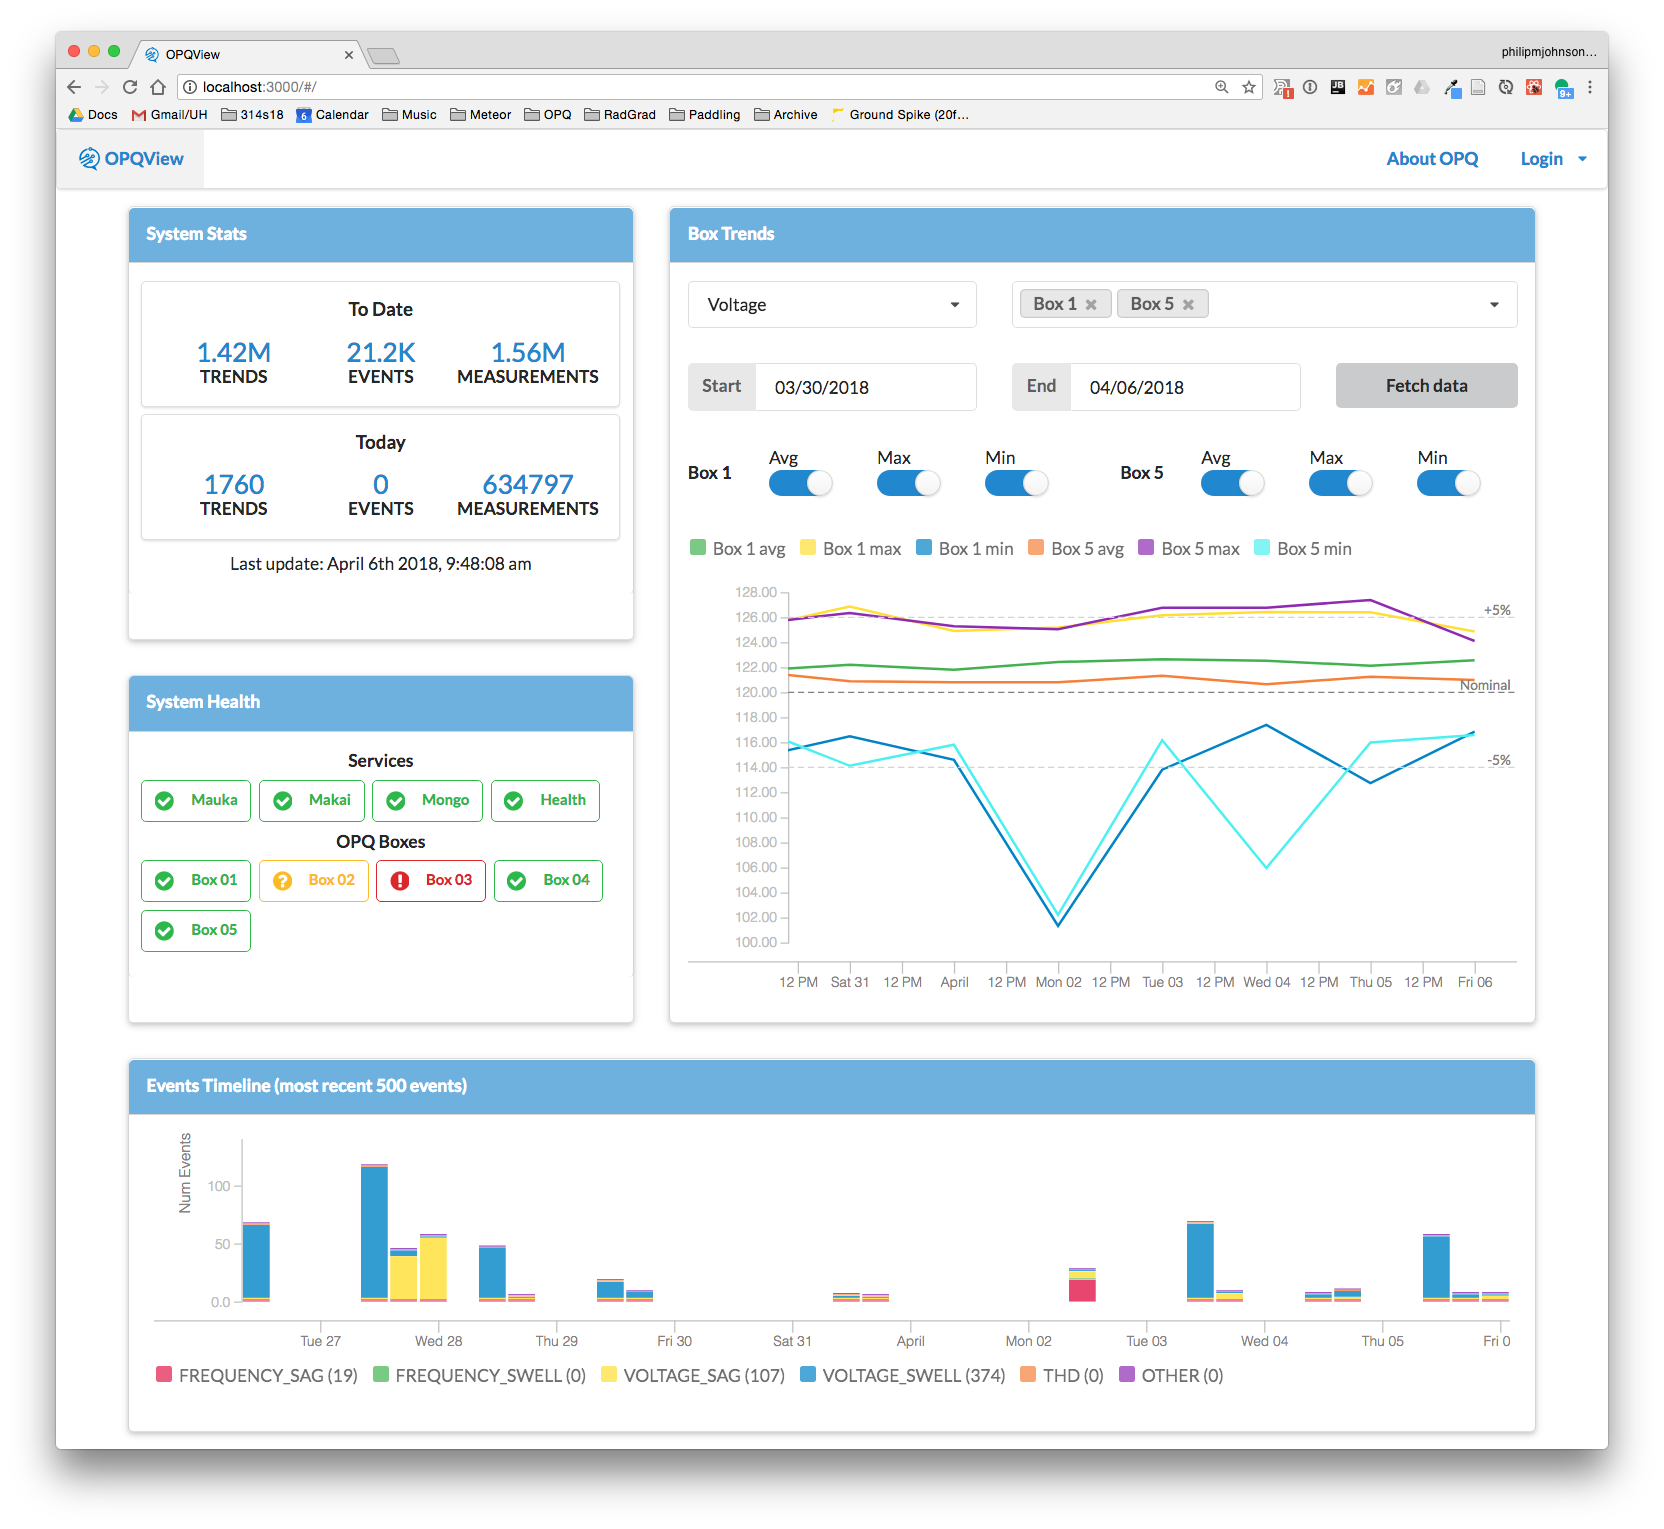
\includegraphics[width=0.6\textwidth]{img/opqview-landing-page.png}
  \end{center}
  \caption{Screenshot of a recent OPQ View build.}
  \label{fig:opq:12}
\end{figure}
